%% -*- coding: utf-8 -*-
\documentclass[12pt,a4paper]{scrartcl} 
\usepackage[utf8]{inputenc}
\usepackage[english,russian]{babel}
\usepackage{indentfirst}
\usepackage{misccorr}
\usepackage{graphicx}
\usepackage{amsmath}
\usepackage{listings}
\usepackage{xcolor}
\usepackage{listings}
\usepackage{xcolor}
\usepackage{float}

\lstdefinestyle{cs-style}{
  language=[Sharp]C,
  basicstyle=\ttfamily\small,
  keywordstyle=\color{blue}\bfseries,
  commentstyle=\color{gray},
  stringstyle=\color{red},
  numbers=left,
  numberstyle=\tiny,
  numbersep=5pt,
  frame=single,
  breaklines=true,
  tabsize=4,
  showstringspaces=false
}

\begin{document}
	\begin{titlepage}
		\begin{center}
			\large
			МИНИСТЕРСТВО НАУКИ И ВЫСШЕГО ОБРАЗОВАНИЯ РОССИЙСКОЙ ФЕДЕРАЦИИ
			
			Федеральное государственное бюджетное образовательное учреждение высшего образования
			
			\textbf{АДЫГЕЙСКИЙ ГОСУДАРСТВЕННЫЙ УНИВЕРСИТЕТ}
			\vspace{0.25cm}
			
			Инженерно-физический факультет
			
			Кафедра автоматизированных систем обработки информации и управления
			\vfill

			\vfill
			
			\textsc{Отчет по практике}\\[5mm]
			
			{\LARGE Программаная реализация численного метода \textit{Найти определитель матрицы}}
			\bigskip
			
			1 курс, группа 1ИВТ АСОИУ
		\end{center}
		\vfill
		
		\newlength{\ML}
		\settowidth{\ML}{«\underline{\hspace{0.7cm}}» \underline{\hspace{2cm}}}
		\hfill\begin{minipage}{0.5\textwidth}
			Выполнил:\\
			\underline{\hspace{\ML}} A.\,Ю.~Федосеев\\
			«\underline{\hspace{0.7cm}}» \underline{\hspace{2cm}} 2025 г.
		\end{minipage}%
		\bigskip

            \newlength{\ML}
		\settowidth{\ML}{«\underline{\hspace{0.7cm}}» \underline{\hspace{2cm}}}
		\hfill\begin{minipage}{0.5\textwidth}
			Выполнил:\\
			\underline{\hspace{\ML}} М.\,А.~Ситимов\\
			«\underline{\hspace{0.7cm}}» \underline{\hspace{2cm}} 2025 г.
		\end{minipage}%
		\bigskip

            \newlength{\ML}
		\settowidth{\ML}{«\underline{\hspace{0.7cm}}» \underline{\hspace{2cm}}}
		\hfill\begin{minipage}{0.5\textwidth}
			Выполнил:\\
			\underline{\hspace{\ML}} В.\,С.~Грицков\\
			«\underline{\hspace{0.7cm}}» \underline{\hspace{2cm}} 2025 г.
		\end{minipage}%
		\bigskip
		
		\hfill\begin{minipage}{0.5\textwidth}
			Руководитель:\\
			\underline{\hspace{\ML}} С.\,В.~Теплоухов\\
			«\underline{\hspace{0.7cm}}» \underline{\hspace{2cm}} 2025 г.
		\end{minipage}%
		\vfill
		
		\begin{center}
			Майкоп, 2025 г.
		\end{center}
	\end{titlepage}

    \section{Введение}
\label{sec:intro}
\subsection{Текстовая формулировка задачи (Вариант 7)}
Найти определитель матрицы.

\subsection{Теория метода}

Определителем квадратной матрицы 
\[
A = \begin{pmatrix}
a_{11} & a_{12} \\
a_{21} & a_{22}
\end{pmatrix}
\]
второго порядка называется число
\[
|A| = a_{11}a_{22} - a_{12}a_{21}.
\]

Определителем 
\[
A = \begin{pmatrix}
a_{11} & \cdots & a_{1n} \\
\vdots & \ddots & \vdots \\
a_{n1} & \cdots & a_{nn}
\end{pmatrix}
\]
квадратной матрицы порядка \( n,\, n \geq 3 \), называется число
\[
|A| = \sum_{k=1}^{n} (-1)^{k+1} a_{1k} M_k,
\]
где \( M_k \) — определитель матрицы порядка \( n-1 \), полученной из матрицы \( A \) вычеркиванием первой строки и столбца с номером \( k \).

\section{Ход работы}
\label{sec:exp}

\subsection{Выбор средств для разработки}
\label{sec:exp:selection}
Для разработки программы, предназначенной для вычисления определителя матрицы, нами был выбран стек технологий, включающий язык программирования C#, платформу .NET Core и фреймворк WPF (Windows Presentation Foundation) для построения пользовательского интерфейса. Этот выбор позволяет создать современное, производительное и кроссплатформенное настольное приложение с гибким и интуитивно понятным интерфейсом. Использование паттерна MVVM обеспечивает четкое разделение представления, бизнес-логики и модели данных, что значительно упрощает разработку, тестирование и сопровождение программы. Язык C# предоставляет возможности строгой типизации и объектно-ориентированного подхода, а WPF — удобные средства визуализации, включая систему привязок данных, шаблоны элементов управления и поддержку стилей, что делает интерфейс приложения более удобным и наглядным для пользователя.

\subsection{Код приложения}
\label{sec:exp:code}
Для упрощения разработки было создано несколько вспомогательных классов. Листинг кода для этих классов приведён ниже:

\lstinputlisting[
  caption=Класс MatrixCalculate для вычисления определителя,
  label={lst:matrix-calc},
  style=cs-style
]{src/MatrixCalculate.cs}

\lstinputlisting[
  caption=Модель одной ячейки матрицы,
  label={lst:matrix-cell-model},
  style=cs-style
]{src/MatrixCellModel.cs}

\lstinputlisting[
  caption=Модель всей матрицы,
  label={lst:matrix-model},
  style=cs-style
]{src/MatrixModel.cs}

\section{Скриншоты программы}
\label{sec:program-shots}

Пример внешнего вида программы представлен на рис.~\ref{fig:pic1}, рис.~\ref{fig:pic2} и рис.~\ref{fig:pic3}.

\begin{figure}[H]
	\centering
	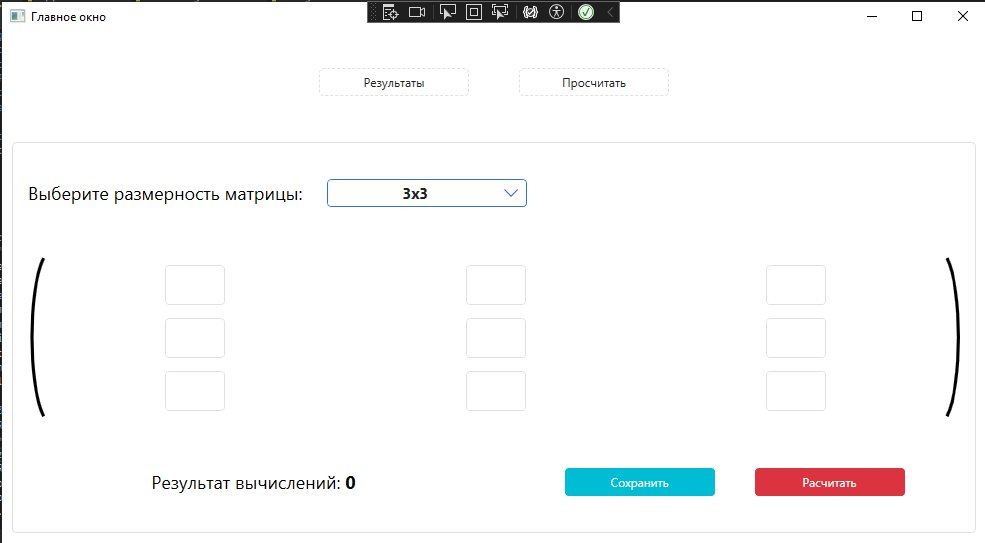
\includegraphics[width=0.5\textwidth,height=6cm,keepaspectratio]{./assets/pic1.jpeg}
	\caption{Страница для заполнения и расчета элементов матрицы}
	\label{fig:pic1}
\end{figure}

\begin{figure}[H]
\centering
\begin{minipage}{0.48\textwidth}
    \centering
    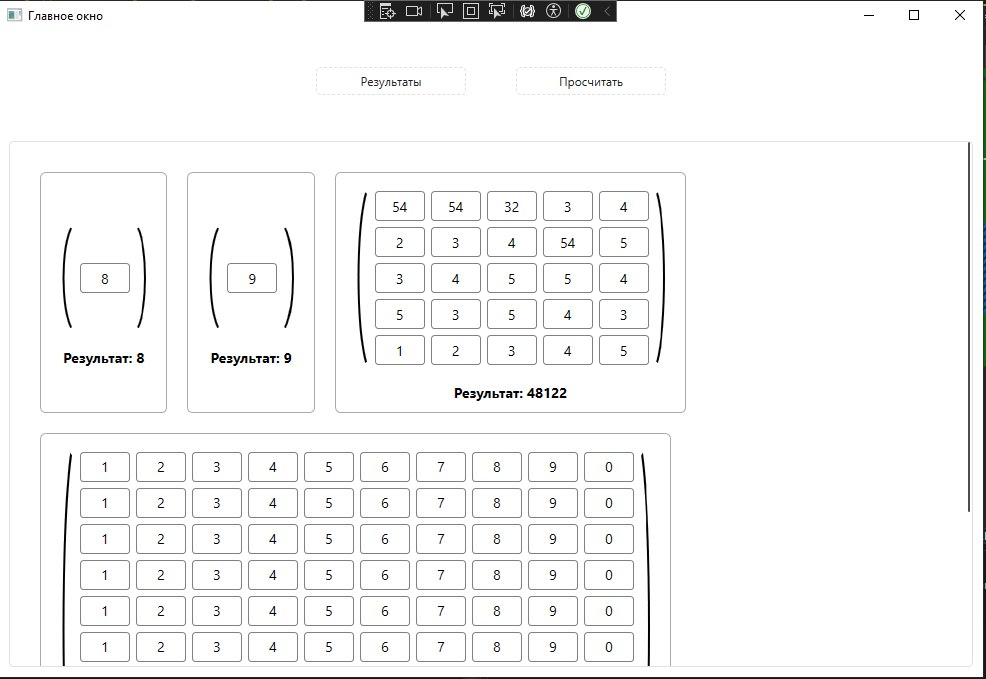
\includegraphics[width=\textwidth]{./assets/pic2.jpeg}
    \caption{Страница для просмотра результатов расчётов (1)}
    \label{fig:pic2}
\end{minipage}
\hfill
\begin{minipage}{0.48\textwidth}
    \centering
    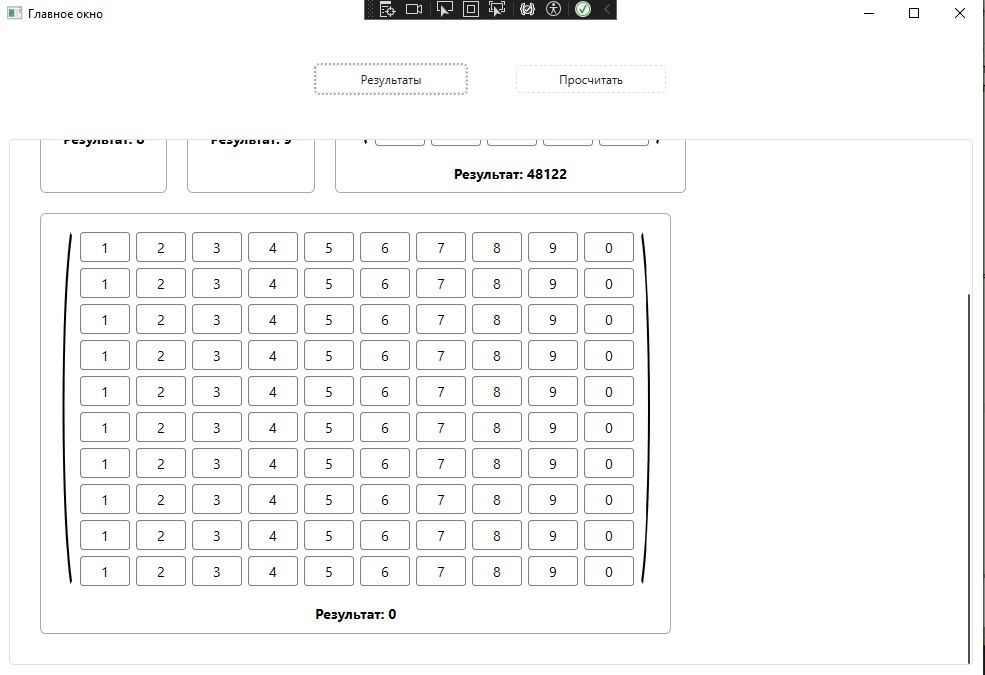
\includegraphics[width=\textwidth]{./assets/pic3.jpeg}
    \caption{Страница для просмотра результатов расчётов (2)}
    \label{fig:pic3}
\end{minipage}
\end{figure}

\section{Источники}
\begin{thebibliography}{9}
\bibitem{Knuth-2003}
Кнут Д.Э. Всё про \TeX. \newblock — Москва: Изд. Вильямс, 2003. — 550~с.
\bibitem{Lvovsky-2003}
Львовский С.М. Набор и верстка в системе \LaTeX{}. \newblock — 3-е издание, исправленное и дополненное, 2003.
\bibitem{Voroncov-2005}
Воронцов К.В. \LaTeX{} в примерах. — 2005.
\bibitem{dotnet-docs}
Документация по платформе .NET. \newblock — \url{https://learn.microsoft.com/dotnet/}, 2024.
\bibitem{csharp-docs}
Документация по языку программирования C\#. \newblock — \url{https://learn.microsoft.com/dotnet/csharp/}, 2024.
\bibitem{wpf-docs}
Официальная документация WPF. \newblock — \url{https://learn.microsoft.com/dotnet/desktop/wpf/}, 2024.
\bibitem{mvvm-pattern}
MVVM Pattern. Архитектура приложений WPF. \newblock — \url{https://learn.microsoft.com/dotnet/architecture/mvvm/}, 2024.
\bibitem{math-theory}
Бронштейн И.Н., Семендяев К.А. Справочник по математике для инженеров и студентов вузов. \newblock — М.: Наука, 1986.
\end{thebibliography}


\end{document}
